\documentclass[a4paper,11pt]{article} % добавить leqno в [] для нумерации слева

%%% Работа с русским языком
\usepackage{cmap}					% поиск в PDF
\usepackage{mathtext} 				% русские буквы в фомулах
\usepackage[T2A]{fontenc}			% кодировка
\usepackage[utf8]{inputenc}			% кодировка исходного текста
\usepackage[english]{babel}	% локализация и переносы
\usepackage[a4paper, total={17cm, 26cm}]{geometry}
\usepackage{multicol}
\usepackage{graphicx}
\usepackage{hyperref}

%%% Дополнительная работа с математикой
\usepackage{amsmath,amsfonts,amssymb,amsthm,mathtools} % AMS
\usepackage{icomma} % "Умная" запятая: $0,2$ --- число, $0, 2$ --- перечисление

%% Номера формул
\mathtoolsset{showonlyrefs=false} % Показывать номера только у тех формул, на которые есть \eqref{} в тексте.

%% Шрифты
\usepackage{euscript}	 % Шрифт Евклид
\usepackage{mathrsfs} % Красивый матшрифт
%\usepackage{pythonhighlight}
\usepackage{underscore}

%% Свои команды
\DeclareMathOperator{\sgn}{\mathop{sgn}}

%% Перенос знаков в формулах (по Львовскому)
\newcommand*{\hm}[1]{#1\nobreak\discretionary{}
{\hbox{$\mathsurround=0pt #1$}}{}}

%%% Заголовок
\author{Kevyn Collins-Thompson\\University of Michigan}
\title{Applied Machine Learning in Python\\Module 4. Supervised Machine Learning --- Part 2}
\date{}

\begin{document} % конец преамбулы, начало документа

\maketitle

\tableofcontents

\vspace{1cm}

\begin{multicols}{2}

\section{Naive Bayes Classifiers}
\begin{multicols}{2}

Another family of supervised learning models that's related to linear classification models is the Naive Bayes family of classifiers, which are based on simple \emph{probabilistic} models of how the data in each class might have been generated. 

Naive Bayes classifiers are called naive because informally, they make the \emph{simplifying assumption} that each feature of an instance is independent of all the others, given the class. 

In practice, of course, this is not often the case, features often are somewhat correlated. For example, in predicting whether a house is likely to sell above the owner's asking price. Some features, such as the are of the interior rooms are likely to be correlated with other features, such as the size of the land that the house is built on or the number of bedrooms. And these features in turn might be correlated with the location of the property, and so on. 

This naive simplifying assumption means on the one hand, that learning a Naive Bayes classifier is \emph{very fast}. Because only simple per class statistics need to be estimated for each feature and applied for each feature independently. 

On the other hand, the penalty for this efficiency is that the \emph{generalization performance} of Naive Bayes Classifiers can often be a bit worse than other more sophisticated methods, or even linear models for classification. 

Even so, especially for high dimensional data sets, Naive Bayes Classifiers can achieve \emph{performance} that's often competitive to other more sophisticated methods, like support vector machines, for some tasks. 

There are three flavors of Naive Bayes Classifier that are available in scikit learn.

\subsection{Bernoulli Naive Bayes model}

The Bernoulli Naive Bayes model uses a set of \emph{binary} occurrence features. When classifying texts document for example, the Bernoulli Naive Bayes model is quit handy because we could represent the presence or the absence of the given word in the text with the binary feature. 

Of course this doesn't take into account how often the word occurs in the text. 

\subsection{Multinomial Naive Bayes model}

So the Multinomial Naive Bayes model uses a set of count base \emph{discrete} features each of which does account for how many times a particular feature such as a word is observed in training example like a document. 

In this lecture we won't have time to cover the Bernoulli or Multinomial Naive Bayes models. However, those models are particularly well suited to textual data, where each feature corresponds to an observation for a particular word. And so you'll see Naive Bayes again, including the Bernoulli and Multinomial models in more depth in the text mining part of this specialization. 

\subsection{Gaussian Naive Bayes model}

This lecture will focus on Gaussian Naive Bayes classifiers which assume features that are \emph{continuous or real-valued}. During training, the Gaussian Naive Bayes Classifier estimates for each feature the \texttt{mean} and \texttt{standard deviation} of the feature value for each class. 

For prediction, the classifier compares the features of the example data point to be predicted with the feature statistics for each class and selects the class that best matches the data point. 

More specifically, the Gaussian Naive Bayes Classifier assumes that the data for each class was generated by a simple class specific \emph{Gaussian distribution}. 

Predicting the class of a new data point corresponds mathematically to estimating the probability that each classes Gaussian distribution was most likely to have generated the data point. Classifier then picks the class that has the highest probability. 

Without going into the mathematics involved, it can be shown that the decision boundary between classes in the two class Gaussian Naive Bayes Classifier. In general is a \emph{parabolic} curve between the classes. 

And in the special case where the variance of these feature is the same for both classes. The decision boundary will be linear. 

Here's what that looks like, typically, on a simple binary classification data set. 

The gray ellipses given idea of the shape of the Gaussian distribution for each class, as if we were looking down from above. 

You can see the centers of the Gaussian's correspond to the mean value of each feature for each class. 

More specifically, the gray ellipses show the contour line of the Gaussian distribution for each class, that corresponds to about two standard deviations from the mean. 

\begin{center}
	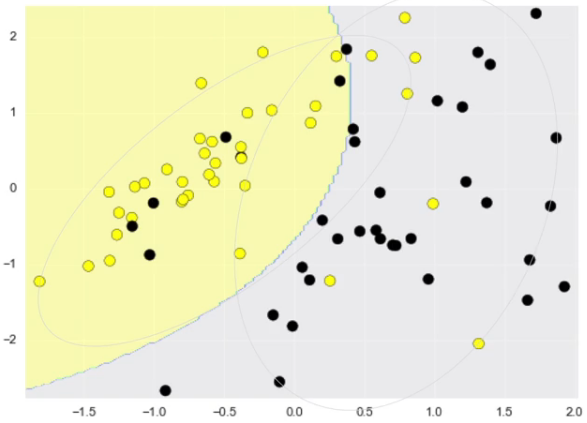
\includegraphics[width=\linewidth]{img/Gaussian-Naive-Bayes-Classifier-1.png} 
\end{center}


The line between the yellow and gray background areas represents the decision boundary. And we can see that this is indeed parabolic. 

To use the Gaussian Naive Bayes classifier in Python, 
we just instantiate an instance of the Gaussian NB class and call the fit method on the training data just as we would with any other classifier. 

\begin{verbatim}
from sklearn.naive_bayes import GaussianNB
\end{verbatim}

\textbf{Note:} the Naive Bayes models are among a few classifiers in scikit learn that support a method called \texttt{partial_fit},  which can be used instead of \texttt{fit} to train the classifier \emph{incrementally} in case you're working with a huge data set that doesn't fit into memory. 

For the \texttt{GaussianNB} class there are no special parameters to control the models complexity. 

Looking at one example in the notebook from our synthetic two class dataset, we can see that, in fact, the Gaussian Naive Bayes classifier achieves quite good performance on this simple classification example. When the classes are no longer as easily separable as with this second, more difficult binary example here. Like linear models, Naive Bayes does not perform as well. 

On a real world example, using the breast cancer data set, the Gaussian Naive Bayes Classifier also does quite well, being quite competitive with other methods, such as support vector classifiers. 

{\scriptsize
\begin{verbatim}
X_train, X_test, y_train, y_test = 
train_test_split(X_cancer, y_cancer, random_state = 0)

nbclf = GaussianNB().fit(X_train, y_train)
print('Breast cancer dataset')
print('Accuracy of GaussianNB classifier on training 
  set: {:.2f}'.format(nbclf.score(X_train, y_train)))
print('Accuracy of GaussianNB classifier on test set:
 {:.2f}'.format(nbclf.score(X_test, y_test)))

Breast cancer dataset
Accuracy of GaussianNB classifier on training set: 0.95
Accuracy of GaussianNB classifier on test set: 0.94
\end{verbatim}
}

Typically, Gaussian Naive Bayes is used for \emph{high-dimensional} data, when each data instance has hundreds, thousands or maybe even more features. Likewise the Bernoulli and Nultinomial flavors of Naive Bayes are used for text classification where there are very large number of distinct words is features and where the future vectors are sparse because any given document uses only a small fraction of the overall vocabulary. 

The Naive Bayes Classifiers are related mathematically to linear models, so many of the pros and cons of linear models also apply to Naive Bayes. 

On the \textbf{positive} side Naive Bayes classifiers are:
\begin{itemize}
\item easy to understand;
\item fast to train and use for prediction;
\item well suitable to high dimensional data including text and the applications involving very large data sets, where efficiency is critical and computational costs rule out other classification approaches;
\item often useful as a baseline comparison against more sophisticated methods.
\end{itemize}


On the \textbf{negative} side:
\begin{itemize}
\item assumption that features are conditionally independence are not realistic; for many real world datasets there's significant covariance among features;
\item other classifier types often have better generalization performance;
\item confidence estimates for predictions are not very accurate.
\end{itemize}

Other more sophisticated classification methods that can account for these dependencies are likely to outperform Naive Bayes. 

And on a side note, when getting confidence or probability estimates associated with predictions, Naive Bayes classifiers produce unreliable estimates, typically. 

Still, Naive Bayes Classifiers can perform very competitively on some tasks, and are also often very useful as baseline models against which more sophisticated models can be compared. 

\end{multicols}

\section{Random Forests}
\begin{multicols}{2}

A widely used and effective method in machine learning involves creating learning models known as \emph{ensembles}. An ensemble takes multiple individual learning models and combines them to produce an aggregate model that is more powerful than any of its individual learning models alone. 

Why are ensembles effective? Well, one reason is that if we have different learning models, although each of them might perform well individually, they'll tend to make different kinds of mistakes on the data set. And typically, this happens because each individual model might overfit to a different part of the data. By combining different individual models into an ensemble, we can average out their individual mistakes to reduce the risk of overfitting while maintaining strong prediction performance. 

Random forests are an example of the ensemble idea applied to decision trees. Random forests are widely used in practice and achieve very good results on a wide variety of problems. They can be used as classifiers via the sklearn \texttt{RandomForestClassifier} class or for regression using the \texttt{RandomForestRegressor} class both in the \texttt{sklearn.ensemble} module. 

As we saw earlier, one disadvantage of using a \emph{single} decision tree was that decision trees tend to be prone to overfitting the training data. 

As its name would suggest, a random forest creates lots of individual decision trees on a training set, often on the order of tens or hundreds of trees. The idea is that each of the individual trees in a random forest should do reasonably well at predicting the target values in the training set but should also be constructed to be different in some way from the other trees in the forest. 

Again, as the name would suggest this difference is accomplished by introducing random variation into the process of building each decision tree. 

\begin{center}
	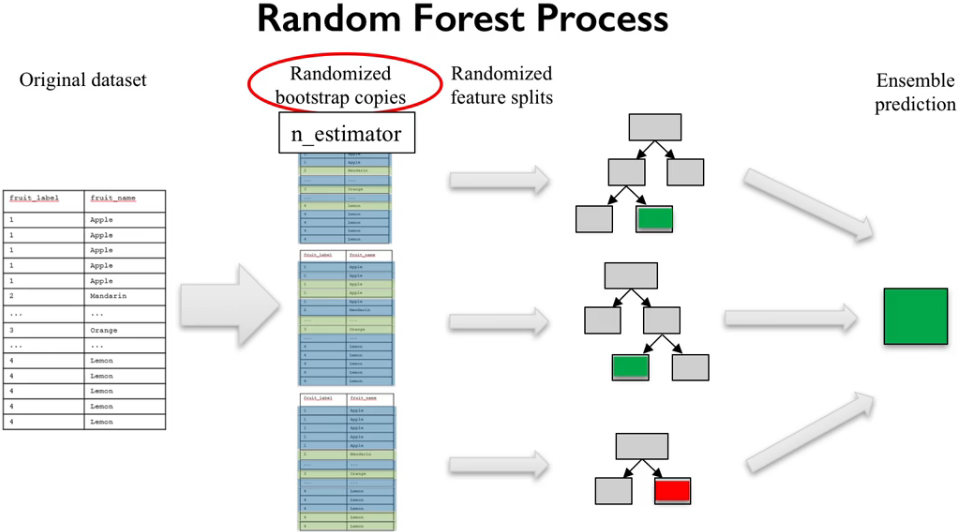
\includegraphics[width=\linewidth]{img/Random-Forest-Process.png} 
\end{center}


This random variation during tree building happens in two ways. First, the data used to build each tree is selected randomly and second, the features chosen in each split tests are also randomly selected. 

\subsection{Random Forests Model Creation}

To create a random forest model you first decide on how many trees to build. This is set using the \texttt{n_estimated} parameter for both RandomForestClassifier and RandomForestRegressor. Each tree were built from a different random sample of the data called the bootstrap sample. Bootstrap samples are commonly used in statistics and machine learning. If your training set has N instances or samples in total, a bootstrap sample of size N is created by just repeatedly picking one of the N dataset rows at random with replacement, that is, allowing for the possibility of picking the same row again at each selection. 

\begin{center}
	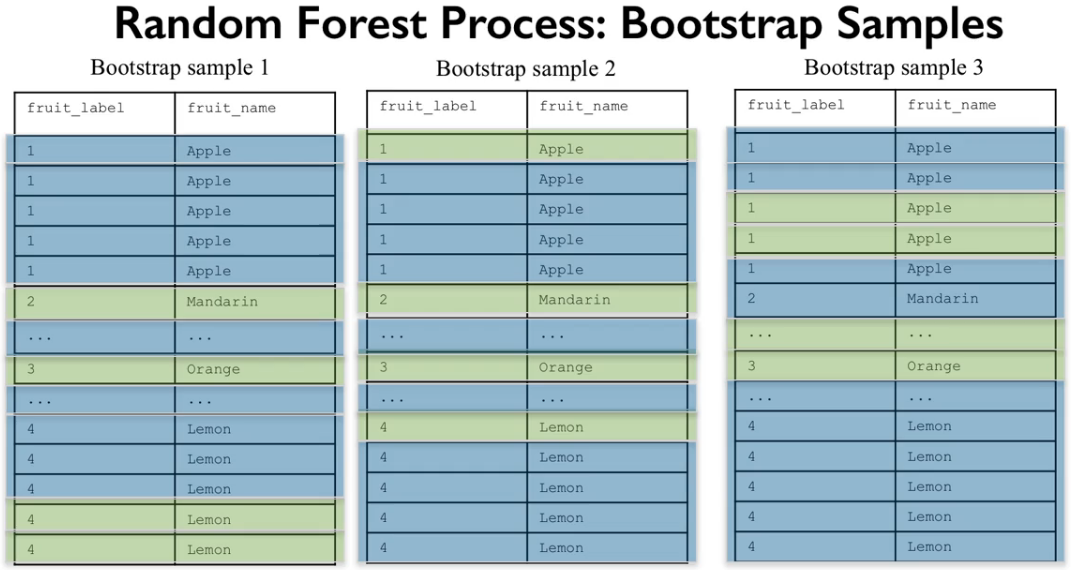
\includegraphics[width=\linewidth]{img/Bootstrap-Samples.png} 
\end{center}

You repeat this random selection process N times. The resulting bootstrap sample has N rows just like the original training set but with possibly some rows from the original dataset missing and others occurring multiple times just due to the nature of the random selection with replacement. 

When building a decision tree for a random forest, the process is almost the same as for a standard decision tree but with one important \emph{difference}. When picking the best split for a node, instead of finding the best split across all possible features, a \emph{random subset of features} is chosen and the best split is found within that smaller subset of features. The number of features in the subset that are randomly considered at each stage is controlled by the \texttt{max_features} parameter. 

This randomness in selecting the bootstrap sample to train an individual tree in a forest ensemble, combined with the fact that splitting a node in the tree is restricted to random subsets of the features of the split, virtually guarantees that all of the decision trees and the random forest will be different. 

The random forest model is quite sensitive to the \texttt{max_features} parameter. If \texttt{max_features = 1}, the random forest is limited to performing a split on the single feature that was selected randomly instead of being able to take the best split over several variables. This means the trees in the forest will likely be very different from each other and possibly with many levels in order to produce a good fit to the data. 

On the other hand if \texttt{max_features} is high, close to the total number of features that each instance has, the trees in the forest will tend to be similar and probably will require fewer levels to fit the data using the most informative features. 

\subsection{Prediction}

Once a random forest model is trained, it predicts the target value for new instances by first making a prediction for every tree in the random forest. 

\begin{center}
	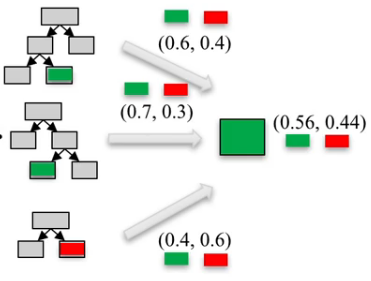
\includegraphics[width=\linewidth]{img/Random-Forest-Prediction.png} 
\end{center}

For \emph{regression} tasks the overall prediction is then typically the \textbf{mean} of the individual tree predictions. For \emph{classification} the overall prediction is based on a \textbf{weighted vote}. Each tree gives a probability for each possible target class label then the probabilities for each class are averaged across all the trees and the class with the highest probability is the final predicted class. 

\begin{center}
	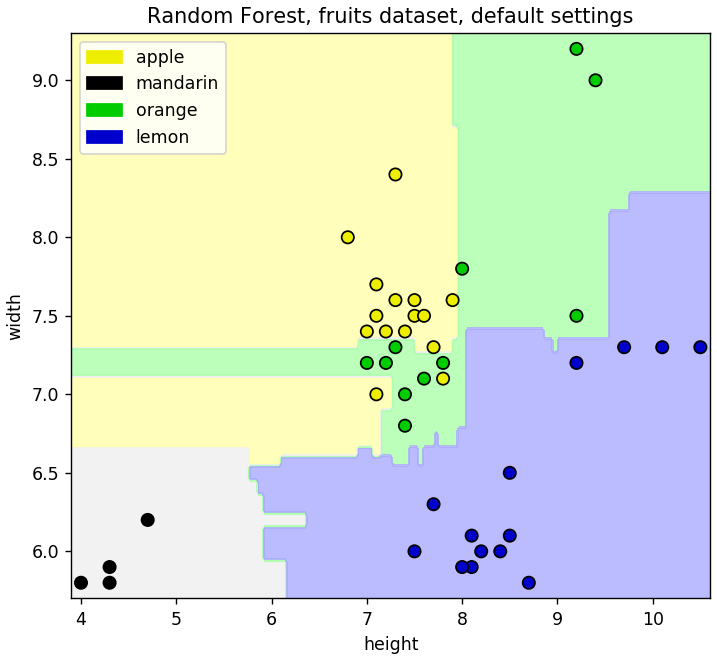
\includegraphics[width=\linewidth]{img/Random-Forest-Fruit-dataset.png} 
\end{center}

Here's an example of learning a random forest of the example fruit dataset using two features, height and width. Here we're showing the training data plotted in terms of two feature values with height on the x axis and width on the y axis. 

As usual, there are four categories of fruit to be predicted. Because the number of features is restricted to just two in this very simple example, the randomness in creating the tree ensemble is coming mostly from the bootstrap sampling of the training data. You can see that the decision boundaries overall have the \emph{box like shape} that we associate with decision trees but with some additional detail variation to accommodate specific local changes in the training data. 

Overall, you can get an impression of the increased complexity of this random forest model in capturing both the global and local patterns in the training data compared to the single decision tree model we saw earlier. 

\subsection{Implementation}

\subsubsection*{Fruit dataset}

Let's take a look at the notebook code that created and visualized this random forest on the fruit dataset.
{\scriptsize
\begin{verbatim}
from sklearn.ensemble import RandomForestClassifier
...
clf = RandomForestClassifier().fit(X, y)
clf = RandomForestClassifier(n_estimators = 10,
      random_state=0).fit(X_train, y_train)
...
Random Forest, Fruit dataset, default settings
Accuracy of RF classifier on training set: 1.00
Accuracy of RF classifier on test set: 0.80
\end{verbatim}
}

To use the \texttt{RandomForestClassifier} we import the random forest classifier class from the \texttt{sklearn.ensemble} library. 

For each pair of features we call the fit method on that subset of the training data X using the labels y. We then use the utility function plot class regions for classifier to visualize the training data and the random forest decision boundaries. 

Let's apply random forest to a larger dataset with more features. 

\subsubsection*{Breast Cancer dataset}

For comparison with other supervised learning methods, we use the breast cancer dataset. We create a new random forest classifier and since there are about 30 features, we'll set \texttt{max_features~=~8} to give a diverse set of trees that also fit the data reasonably well. 

{\scriptsize
\begin{verbatim}
Breast cancer dataset
Accuracy of RF classifier on training set: 1.00
Accuracy of RF classifier on test set: 0.99
\end{verbatim}
}

We can see that random forest with no feature scaling or extensive parameter tuning achieve very good test set performance on this dataset, in fact, it's as good or better than all the other supervised methods we've seen so far including current life support vector machines and neural networks that require more careful tuning. 

\textbf{Notice} that we did not have to perform scaling or other pre-processing as we did with a number of other supervised learning methods. This is one \emph{advantage} of using random forests. 

\subsection{Pros and Cons}

On the \textbf{positive} side of Random Forests:
\begin{itemize}
\item widely used, excellent prediction performance on many problems;
\item doesn't require careful normalization of features or extensive paramener tuning;
\item like decision trees, handles a mixture of feature types;
\item easily parallelized across multiple CPUs.
\end{itemize}

Even though building many different trees requires a corresponding increase in computation, building random forests is easily parallelized across multiple CPU's. 


On the \textbf{negative} side:
\begin{itemize}
\item the resulting modela are often difficult for humans to interpret~--- difficult to see the predictive structure of the features or to know why a particular prediction was made;
\item not a good choice for tasks that have very high dimensional sparse features like text classification.
\end{itemize}

\subsection{Key Parameters}

Here are some of the key parameters that you'll need for using random forests. 

\texttt{N_estimators} sets the number of trees to use. The default value for \texttt{n_estimators}~= 10 and increasing this number for larger data sets is almost certainly a good idea since ensembles that can average over more trees will reduce overfitting. 

Just bear in mind that increasing the number of trees in the model will also increase the computational cost of training. You'll use more time and more memory. So in practice you'll want to choose the parameters that make best use of the resources available on your system. 

The \texttt{max_features} parameter has a strong effect on performance. It has a large influence on how diverse the random trees in the forest are. Typically, the default setting of \texttt{max_features}, which for classification is the square root of the total number of features and for regression is the log base two of the total number of features, works quite well in practice although explicitly adjusting \texttt{max_features} may give you some additional performance gain with smaller values of max features tending to reduce overfitting. 

The \texttt{max_depth} parameter controls the depth of each tree in the ensemble. The default setting for this is none, in other words, the nodes in a tree will continue to be split until all leaves contain the same class or have fewer samples than the minimum sample split parameter value, which is two by default. 

The \texttt{n_jobs} parameter~--- how many cores to use in parallel to train the model. Generally, you can expect something close to a linear speed up. So, for example, if you have four cores, the training will be four times as fast as if you just used one. If you set end jobs to negative one it will use all the cores on your system and setting end jobs to a number that's more than the number of cores on your system won't have any additional effect. 

\end{multicols}

%\section{Classifier Decision Functions}
\begin{multicols}{2}

Many classifiers in scikit learn can provide information about the uncertainty associated with a particular prediction either by using the \textbf{decision function} method or the \textbf{predict proba} method. 

\subsection{Decision function method}

When given a set of test points, the decision function method provides for each one a classifier score value that indicates how confidently classifier predicts the positive class. So there will be large magnitude positive scores for those points, or it predicts a negative class, there'll be large magnitude negative scores for negative points. 

Here's an example in the notebook showing the first few instances from our classification problem using a logistic regression classifier. We can see the instances in the negative class often have large magnitude negative scores. And indeed the instances in the positive class has positive scores from the logistic regression classifier. 

\subsection{Predict proba function}

Likewise, the \texttt{predict_proba} function provides \emph{predicted probabilities} of class membership. 

Typically a classifier would choose the more likely class. That is in a binary classifier, the class with probability greater than 50\%. 

\subsection{Decision threshold}

Adjusting this decision threshold affects the prediction of the classifier. A higher threshold means that a classifier has to be more confident in predicting the class. For example, we might predict class one only if the estimated probability of class one was over 70\%. And this results in a more conservative classifier. 

Here's an example of getting these prediction probabilities for the test instances for the same logistic regression classifier. 

You can see that many entries with a positive label of one, have a high probability like 0.995. While many negative label instances have a very low prediction probability. 

\textbf{Note} that \emph{not all} models provide useful probability estimates of this type. For example, a model that was over-fit to a trending set, might provide overly optimistic high probabilities that were in fact not accurate. 

Now, we can use these decision scores or prediction probabilities for getting more complete evaluation picture of a classifiers performance. For a particular application, we might pick a specific decision threshold depending on whether we want the classifier to be more or less conservative about making false-positive or false-negative errors. 

It might not be entirely clear when developing a new model, what the right decision threshold would be, and how that choice will affect evaluation metrics like precision and recall. So instead, what we'll do is, look at how classifier performs for all possible decision thresholds. 

This example shows how that works. On the left here is a list of test instances with their true label and classifier score. 

\begin{center}
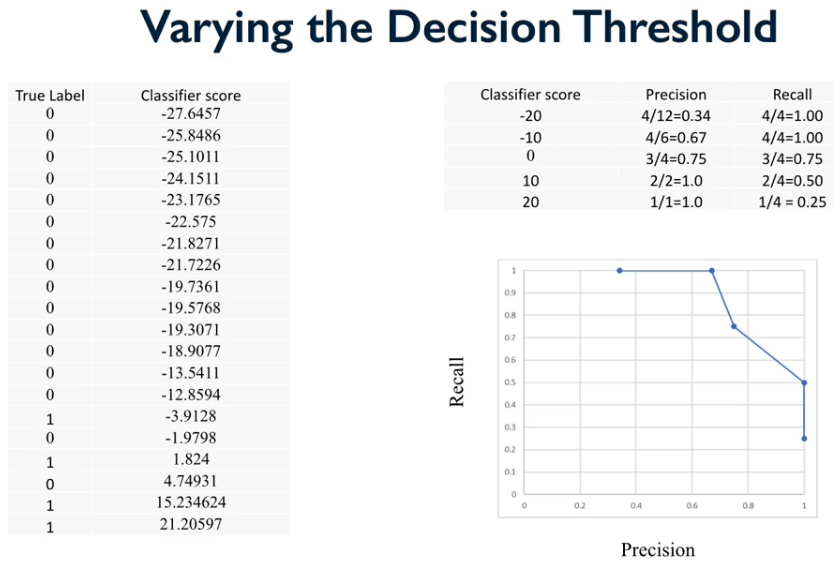
\includegraphics[width=\linewidth]{img/Varying-Decision-Threshold.png} 
\end{center}

If we set a decision threshold, then all the instances above that line, for example if we set the decision threshold to be -20 here. 

Then, all the instances above the line are below the threshold of -20. So -20 or less and all the instances in this direction are above the threshold of -20. And so the ones below the threshold will be predicted to be in the- class. 

And the ones above the threshold will be predicted to be in the + class. 

So, if we pick the specific threshold, so in this case, -20. And we partition the test points in this way. We can compute partition and recall for the points that are predicted to be in the positive class. So in this case, we have 12 instances here, 12 total instances. 

They're being predicted as positive and only four of them, this one, this one, this one, and this one are actually positive and so the precision here is 4 divided by 12 or approximately 0.34. 

The recall on the other hand, there are four positive labeled instances in the whole set of test examples here and we've found all of them with this particular threshold setting. So the recall here is 4 out of 4, we found all four positive labeled examples. And so, for this particular threshold of -20, we can obtain precision on re cost score for that threshold. 

Let's pick a different threshold let's look at what happened when the threshold is -10? Right here, so again anything below this line is treated and has a higher value than -10 here, so those would be treated as + predictions. 

Things above the line have a score below -10, so these would be predicted to be 

And again, we can compute a precision and recall for this decision threshold setting, and we can see here that there are a total of six instances in the + prediction class. Of which four are actually of the positive class, and so the precision here is 4 over 6 or about 0.67. And again, the recall here is going to be 4 out of 4, and it's going to be 1.0. Again, so that corresponds to this point in the table over here. And then as were computing these different precision and recalls for different Thresholds. We can also plot them on this precision recall chart. So the first pair of precision recall numbers that I got, 0.34 and 1.0, we can plot on this point in precision recall space. The second example, so this was for the threshold of -20. 

When the threshold was -10, we got precision of .67 and a recall of 1 corresponding to this point that we can plot. 

And so you can see that if we do this for a number of other thresholds, for example the threshold of 0, we'll get a precision of 0.75. And a recall of 0.75 that corresponds to this point. 

And in that choice of decision threshold. And we can keep doing that for different thresholds. And we actually are plotting a series of points through the space which we can be connected at as a curve. 

And so in this way, we can get a more complete picture by varying the threshold of how the precision and recall of the result and classifier output changes as a function of the decision threshold. 

And this resulting chart here is called a precision recall curve and we'll look at it in more detail next. 

\end{multicols}

%\section{Precision-Recall and ROC curves}
\begin{multicols}{2}

\subsection{Precision-Recall Curves}

Precision-Recall Curves are very widely used evaluation method from machine learning. 

As we just saw in example, the x axis shows precision and the y axis shows recall. 

Now an ideal classifier would be able to achieve perfect precision of 1.0 and perfect recall of 1.0. So the optimal point would be up here in the top right. And in general, with precision recall curves, the closer in some sense, the curve is to the top right corner, the more preferable it is, the more beneficial the tradeoff it gives between precision and recall. And we saw some examples already of how there is a tradeoff between those two quantities, between precision and recall, with many classifiers. 


\begin{center}
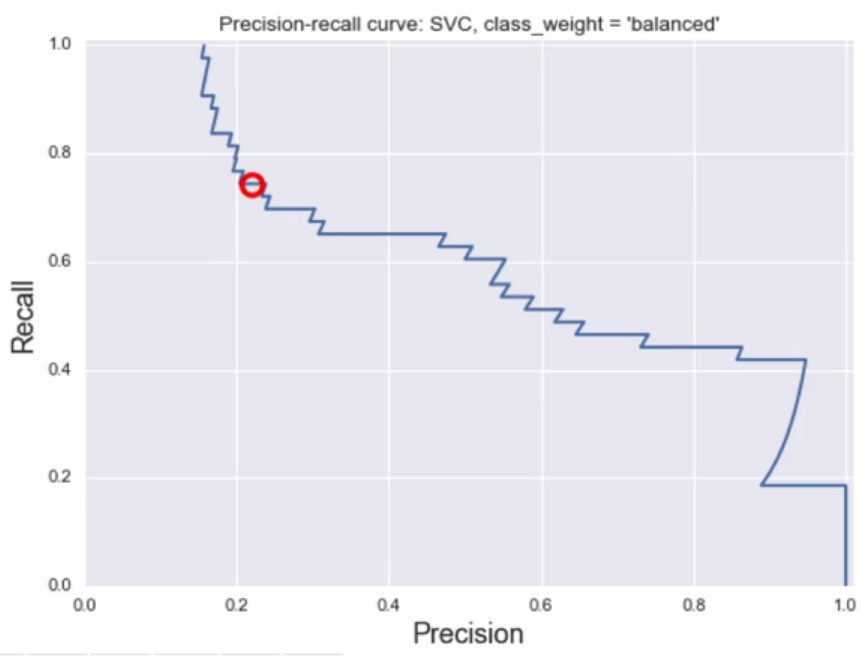
\includegraphics[width=\linewidth]{img/Precision-Recall-curve.png} 
\end{center}

This example here is an actual precision recall curve that we generated using the following notebook code. 

{\scriptsize
\begin{verbatim}
from sklearn.metrics import precision_recall_curve

precision, recall, thresholds = 
    precision_recall_curve(y_test, y_scores_lr)
closest_zero = np.argmin(np.abs(thresholds))
closest_zero_p = precision[closest_zero]
closest_zero_r = recall[closest_zero]

plt.figure()
plt.xlim([0.0, 1.01])
plt.ylim([0.0, 1.01])
plt.plot(precision, recall, label='Precision-Recall Curve')
plt.plot(closest_zero_p, closest_zero_r, 'o', 
    markersize = 12, fillstyle = 'none', c='r', mew=3)
plt.xlabel('Precision', fontsize=16)
plt.ylabel('Recall', fontsize=16)
plt.axes().set_aspect('equal')
plt.show()
\end{verbatim}
}
The red circle indicates the precision and recall that's achieved when the decision threshold is zero. So I created this curve using exactly the same method as we saw in the previous example, by looking at the decision function output from a support vector classifier. Applying varying  decision boundary, looking at how the precision of recall change as the decision boundary changed. Fortunately, scikit-learn has a function that's built in that does all of that, that can compute the precision- recall curve. 

So you can see that in this particular application there is a general downward trend. So as the precision of the classifier goes up, the recall tends to go down. 

In this particular case you'll see also that it's not exactly a smooth curve. There are some jaggy areas and, in fact, the jumps tend to get a little bigger as we approach maximum precision. This is a consequence of how the formulas for precision and recall are computed. They use discrete counts that include the number of true positives. And so as the decision threshold increases, there are fewer and fewer points that remain as positive predictions. So the fractions that are computed for these smaller numbers can change pretty dramatically with small changes in the decision threshold. And that's why these sort of trailing edges of the precision-recall curve can appear a bit jagged when you plot them. 

\subsection{Receiver Operating Characteristic (ROC) curves}

ROC curves or receiver operating characteristic curves are a very widely used visualization method that illustrate the performance of a binary classifier. 

\begin{center}
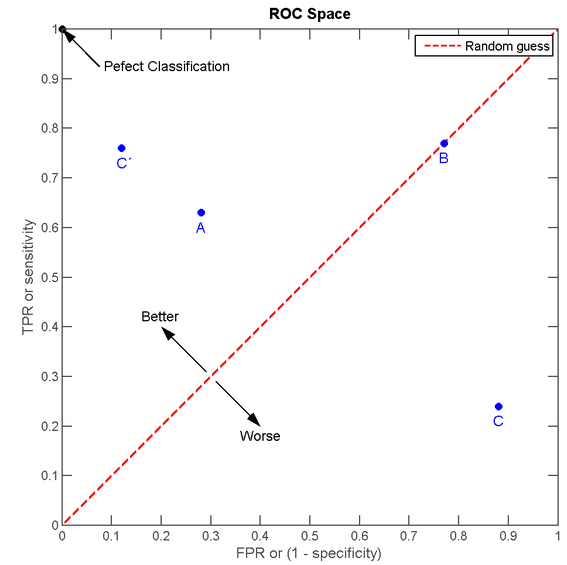
\includegraphics[width=\linewidth]{img/640px-ROC-space-2.png} 
\end{center}



ROC curves on the X-axis show a classifier's False Positive Rate so that would go from 0 to 1.0, and on the Y-axis they show a classifier's True Positive Rate so that will also go from 0 to 1.0. The ideal point in ROC space is one where the classifier achieves zero, a false positive rate of zero, and a true positive rate of one. So that would be the upper left corner. 

So curves in ROC space represent different tradeoffs as the decision boundary, the decision threshold is varied for the classifier. So just as in the precision recall case, as we vary decision threshold, we'll get different numbers of false positives and true positives that we can plot on a chart. 


\begin{center}
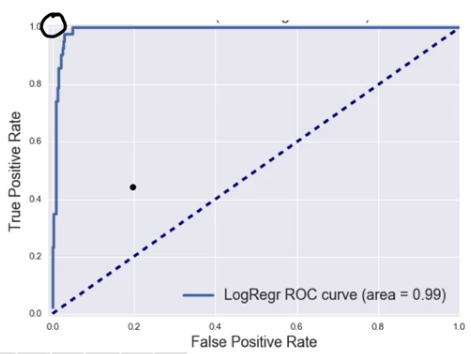
\includegraphics[width=\linewidth]{img/ROC-curve.png} 
\end{center}

The dotted line here that I'm showing is the classifier curve that secretly results from a classifier that randomly guesses the label for a binary class. 

It's basically like flipping a coin. If you have two classes with equal numbers of positive and negative incidences, then flipping a coin will get you randomly equal numbers of false positives and true positives for a large virus data sets. So the dotted line here is used as a base line. So bad classifier will have performance that is random or maybe even worse than random or be slightly better than random. Reasonably good classifier will give an ROC curve that is consistently better than random across all decision threshold choices. 

And then an excellent classifier would be one like I've shown here, which is way up into the left. 

This particular example is an example of a logistic regression classifier using the notebook example you've seen. 

So, the shape of the curve can be important as well, the steepness of the curve, we want classifiers that maximize the true positive rate while minimizing the false positive rate. 

Now as we'll see next, we can qualify the goodness of a classifier in some sense by looking at how much area there is underneath the curve. 

So the area underneath the random classifier is going to be 0.5 but then the area, as you can see, the size of the bumpiness of the classifier as it approaches the top left corner. Well, the area underneath the curve will get larger and larger. It will approach 1. And so, as we'll see in the next slide. 

\subsection{Area Under the ROC Curve (AUC)}

We use something called area under the curve, AUC. That's the single number that measures this total area underneath the ROC curve as a way to summarize a classifier's performance. So, an AUC of zero represents a very bad classifier, and an AUC of one will represent an optimal classifier. In \texttt{Scikit-learn} it is the \texttt{roc_auc_score()}.

\end{multicols}

%\section{Multi-Class Evaluation}
\begin{multicols}{2}

Now that we've looked at evaluation of binary classifiers, let's take a look at how the more general case of multi class classification is handled in evaluation. So in may respects, multi-class evaluation is a straightforward extension of the methods we use in binary evaluation. Instead of two classes, we have multiple classes. So, the results for multi-class evaluation amount to a collection of true verses predicted binary outcome per class. And just as we saw in the binary case, you can generate confusion matrices in the multi-class case. They're especially useful when you have multiple classes, because there are many different kinds of errors that result from one true class being predicted as a different class. We'll look at an example of that. Classification reports that we saw in the binary case are easy to generate for the multi-class case. Now the one area, which is worth a little more examination is how averaging across classes takes place. 

There are different ways to average multi-class results that we'll cover shortly. And the support, the number of instances for each class is important to consider. So just as we're all interested in how to handle imbalance classes in the binary case, it's important as you will see to consider similar issues of how the support for classes might vary to a large or small extent across multiple classes. There is a case of multi-label classification in which each instance could have multiple labels. For example, a web page might be labeled with different topics that come from a predefined set of areas of interest. We won't cover multi-label classification in this lecture. Instead, we'll focus exclusively on multi-class evaluation. The multi-class confusion matrix is a straightforward extension of the binary classifier two by two confusion matrix. 

For example, in our digits data set, there are ten classes for the digits, zero through nine. So, the ten class confusion matrix is a ten by ten matrix with the true digit class indexed by row and the predicted digit class indexed by column. 

As with the two by two case, the correct prediction is by the classifier where the true class matches the predicted class are all along the diagonal and misclassifications are off the diagonal. 

In this example which was created using the following notebook code 

based on a support vector classifier with linear kernel, we can see that most of the predictions are correct with only a few misclassifications here and there. 

The most frequent type of mistake here is apparently misclassifying the true digit, eight as a predicted digit one which happened three times. 

And indeed, the overall accuracy is high, about 97\% as shown here. As an aside, it's sometimes useful to display a confusion matrix as a heat map in order to highlight the relative frequencies of different types of errors. So, I've included the code to generate that here. For comparison, I've also included a second confusion matrix on the same dataset for another support vector classifier that does much worse in a distinctive way. The only change is to use an RBF, radial basis function kernel instead of a linear kernel. 

While we can see for the accuracy number were about 43\% below the confusion matrix that the classifier is doing much worse than the delinear kernel, that single number doesn't give much insight into why. 

Looking at the confusion matrix, however, reveals that for every true digit class, a significant fraction of outcomes are to predict the digit four. That's rather surprising. For example, of the 44 instances of the true digit 2 in row 2, 17 are classified correctly, but 27 are classified as the digit 4. Clearly, something is broken with this model and I picked this second example just to show an extreme example of what you might see when things go quite wrong. This digits dataset is well-established and free of problems. But especially when developing with a new dataset, seeing patterns like this in a confusion matrix could give you valuable clues about possible problems, say in the feature pre-processing for example. So as a general rule of thumb as part of model evaluation, I suggest always looking at the confusion matrix for your classifier. To get some insight into what kind of errors it is making for each class including whether some classes are much more prone to certain kinds of errors than others. 

Next, just as in the binary case, you can get a classification report that summarizes multiple evaluation metrics for a multi-class classifier with an average metric computed for each class. 

Now what I'm about to describe, also applies to the binary class case, but it's easier to see when looking at multi-class classification problem with several classes. 

So, here's an example of how to compute macro-average precision and micro-average precision on a sample dataset that I have extracted from our fruit dataset. In this example, we have three columns where the first column is the true class of an example. The second column is the predictive class from some classifier and the third column is a binary variable that denotes whether the predictive class matches the two class. 

And here, we have in our, this is a multi-class classification problem. 

And so, we have three classes here. We have several instances there, the orange class. We have two instances that are the lemon class and we have two instances that are the apple class. 

So in this first example, we'll compute macro-average precision and the key aspect of macro-average precision is that each class has equal weight. So in this case, each of these classes will contribute one-third weight towards the final macro-average precision value. 

So, there are two steps to compute macro-average precision. The first one is to compute the metric. So in this case, we're going to compute precision within each class. So, let's take a look at the orange class. There are five total examples in the orange class and only one of them was predicted correctly by the classifier. And so, that leads to a precision for the orange class of 1 out of 5 or 0.20. For the second class, the lemon class. There are a total of two instances and only one of them was predicted correctly, and that leads to a precision of one-half or 0.50 for the lemon class. Let's write the precision for each of the classes that we have calculated. 


This was 0.5. 

And for the third class, the apple class. The classifier predicted both of these correctly. So, that's a precision of 2 out of 2 or 1.0. 

That's the first step. We've computed the precision metric within each class. And then in the second step, we simply average across these three to produce the final result, to get our final macro-average precision. And so we can simply compute the average of 0.2, 0.5 and 1 and we get our final macro-average precision for this set of results of 0.57. You'll notice here that no matter how many instances they were in each class, because we computed position within each class first, each class contributes equally to the overall macro-average. So we could have had, for example, a million examples and from the orange class. But that class would have still been weighted equally, because we would have first computed precision for the million orange examples and then that number would still get a third of the weight compared to the other two classes. So, that's macro-average precision. 

Micro-average precision is computed a little differently and it gives each instance in the data results here equal weight. In micro-average precision, we don't compute precision for each class separately. We treat the entire dataset, the entire set of results here as an aggregate outcome. So to compute micro-average precision, we simply look at how many of all the examples. We have nine examples here in total and micro-average precision will simply compute the precision for all the examples, regardless of class in the set of results. So out of these nine instances, we have found that the classifier predicted four of them correctly. 

And so, the micro-average precision is simply computed as 4/9 or 0.44. And you'll notice here that if we had a million instances of the orange class, for example, that with micro-average precision, because each instance has equal weight. That would lead to the orange class contributing many, many more instances to our overall micro-average precision. And so, the effect of micro-average precision is to give classes with a lot more instances much more influence. So, the average here would have been influenced much more by the million orange examples than by the two lemon and apple examples. 

And so, that is the difference between micro and macro-average precision. If the classes have about the same number of instances, macro and micro-average will be about the same. If some classes are much larger, have more instances than others and you want to weight your metric toward the largest ones, use micro-averaging. If you want to weight your metric towards the smallest classes, use macro-averaging. If the micro-average is much lower than the macro-average, then examine the larger classes for poor metric performance. If the macro-average is much lower than the micro-average, then you should examine the smaller classes to see why they have poor metric performance. Here, we use the average parameter on the scoring function. In the first example, we used the precision metric and specify whether we want micro-average precision which is the first case or macro-average precision in the second case. 

In the second example, we use the F1 metric and compute micro and macro-averaged F1. 

Now that we've seen how to compute these metrics, let's take a look at how to use them to do model selection. 

\end{multicols}

%\section{Regression Evaluation}
\begin{multicols}{2}

We saw that for classification, because there were some scenarios like medical diagnostics predictions or costumer facing web site features, where the consequences of false positive were very different than false negatives. It made sense to distinguish these types of errors and do a more detailed analysis. In evaluating classifiers for example we looked at plots like precision recall curves that could show the trade offs a classifier could achieve between making errors of those two types. 

In theory, we could apply the same type of error analysis and more detailed evaluation to regression that we applied for classification. 

For example, we could analyze the regression model's predictions, and categorize errors of one type. Where the regression model's predicted value was much larger than the target value. Compared to a second error type, where the predicted value was much smaller than the target value. 

In practice though it turns out that for most applications of regression, distinguishing between these types of different errors is not as important. 
This simplifies evaluation for regression quite a bit. 

\subsection{$R^2$ score}

In most cases, the default $R^2$ score that's available for regression and psychic learn and that summarizes how well future instances will be predicted. It's adequate for most tasks. 

As a reminder, the $R^2$ score for \emph{perfect predictor} is \textbf{1.0}. And for a predictor that always output the \emph{same constant value}, the $R^2$ score is \textbf{0.0}. 

The $R^2$ score despite the squared in the name that suggests it's always positive does have the potential to go \emph{negative} for bad model fits, such as when fitting non-linear functions to data. 

\subsection{Alternative metrics}

There are a few alternative regression evaluation metrics you should be aware of that work differently than the $R^2$ score. 

\subsubsection{Mean absolute error}

Mean absolute error takes the mean absolute difference between the target and predicted values. In machine running terms this corresponds to the expected value of L1 norm laws. This is sometimes used for example to asses focused outcomes for regression in time series analysis. 

\subsubsection{Mean squared  error}
Mean squared error takes the mean squared difference between the target and predicted values and this corresponds to the expected value of the L2 norm loss. This is widely used for many regression problems and larger errors have correspondingly larger squared contributions to the mean error. 

Like mean absolute error, mean squared error doesn't distinguish between over and under estimates. 

\subsubsection{Median absolute error}

Finally one situation that does arise quite often, is the existence of \emph{outliers} in the data, which can have unwanted influence on the overall $R^2$ or mean squared value. So in those cases, when ignoring outlier is important, you can use the \emph{median} absolute error score, which is robust with the presence of outliers because it uses the median of the error distribution rather than the mean. 

\subsection{Dummy Regressors}

We saw how using how dummy classifiers could give us simple but useful baselines to compared against when evaluating a classifier. The same functionality exist for regression. 

DummyRegressors, as you might guess, are the counterpart to DummyClassifiers for regression. And they serve a similar role as a null outcome baseline and sanity check for regression models. Since regression models have continuous value prediction outputs. The strategy parameter for DummyRegressors gives you a choice of function that you can apply to the distribution of target values found in the training set. You can ask for the mean or median value of the training set targets. The value corresponding to the quantile that you provide or a custom constant value. 

There's a dummy regressor class that provides predictions using simple strategies that do not look at the input data.
 
\begin{center}
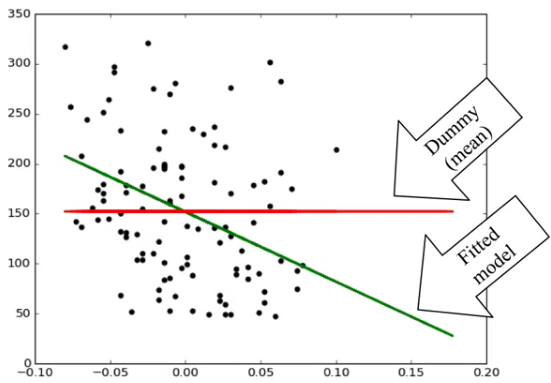
\includegraphics[width=\linewidth]{img/Dummy-Regressor.png}
\end{center}

This example which is available as the regression example from this lecture's notebook shows a scatter plot using database on a single input variable, which is plotted along the x axis from the diabetes data set. 

The points are the data instances from the test split and form a cloud that looks like it may trend down slightly to the right. 

The green line, which is also labeled fitted model is the default linear regression that was fit to the training points. We can see that it’s not a particularly strong fit to the test data. 

The red line labeled dummy mean, shows a linear model that uses the strategy of always predicting the mean of the training data. 

So this is an example of a dummy regressor. 

You can look at the notebook to see that a dummy regressor is created and used just like a regular regression model. You create, fit with the training data, and then call predict on the test data. Although again, like the dummy classifier you \emph{should not} use the dummy regressor for actual problems. Its only use is to provide a baseline for comparison. 

Looking at the regression metrics output from the linear model compared to the dummy model. 

\begin{verbatim}
Linear model, coefficients:[-698.80206267]
Mean squared error (dummy): 4965.13
Mean squared error (linear model): 4646.74
r2_score (dummy): -0.00
r2_score (linear model): 0.06
\end{verbatim}

We can see that as expected the dummy regressor achieves an $R^2$ score of \textbf{0}. Since it always makes a constant prediction without looking at the output. 

In this instance the linear model provides only slightly better fit than the dummy regressor, according to both mean squared error and the $R^2$ score. 

Aside from the strategy of always predicting the mean of the training target values, you could also create some other flavors of dummy regressors that always predict the \emph{median} of the training target values, or a particular \emph{quantile} of those values, or a specific custom \emph{constant value} that you provide. 

Although regression typically has simpler evaluation needs than classification, it does pay to double check to make sure the evaluation metric you choose for a regression problem does penalize errors in a way that reflects the consequences of those errors for the business, organizational, or user needs of your application. 

\end{multicols}

%\section{Model Selection: Optimizing Classifiers for Different Evaluation Metrics}
\begin{multicols}{2}

Now that you've seen a number of different evaluation metrics for both binary and multiclass classification, let's take a look at how you can apply them as criteria for selecting the best classifier for your application, otherwise known as \emph{model selection}. 

In previous lectures we've seen a number of different evaluation frameworks for potential model selection. 

First, we simply did \emph{training and testing on the same dataset}, which as we well know, typically overfits badly and doesn't generalize well to new data. As a side note however, it can serve as a \emph{useful sanity check} to make sure your software engineering and feature generation pipeline is working correctly. 

Second, we frequently use the \emph{train-test split} to produce a single evaluation metric. While fast and easy, this doesn't give as realistic a set of estimates for how well the model may work on future new data. And we don't get a good picture for the variance in the evaluation metrics that may result as we do prediction on different test sets. 

Third, we used \emph{k-fold cross-validation} to create K random train-test splits, where the evaluation metric was averaged across splits. This leads to models that are more reliable on unseen data. 

In particular, we can also use grid search using for example the \texttt{GridSearchCV} method within each cross-validation fold, to find optimal parameters for a model with respect to the evaluation metric.

The default evaluation metric used for a cross-validation score or GridSearchCV is \emph{accuracy}. So how do you apply the new metrics you've learned about here like AUC in model selection? Scikit-learn makes this very easy. You simply add a \texttt{scoring} parameter that's set to the string with the name of the evaluation metric you want to use. 

\subsection{Cross Validation}

Here we're running five folds using a support vector classifier with a linear kernel and C parameter set to one. 

{\scriptsize
\begin{verbatim}
from sklearn.model_selection import cross_val_score
from sklearn.svm import SVC

dataset = load_digits()
# again, making this a binary problem with 'digit 1' 
# as positive class and 'not 1' as negative class
X, y = dataset.data, dataset.target == 1
clf = SVC(kernel='linear', C=1)

# accuracy is the default scoring metric
print('Cross-validation (accuracy)', 
       cross_val_score(clf, X, y, cv=5))
# use AUC as scoring metric
print('Cross-validation (AUC)', 
 cross_val_score(clf, X, y, cv=5, scoring = 'roc_auc'))
# use recall as scoring metric
print('Cross-validation (recall)', 
  cross_val_score(clf, X, y, cv=5, scoring = 'recall'))

Cross-validation (accuracy) 
[0.91944444 0.98611111 0.97214485 0.97493036 0.96935933]
Cross-validation (AUC) 
[0.9641871  0.9976571  0.99372205 0.99699002 0.98675611]
Cross-validation (recall) 
[0.81081081 0.89189189 0.83333333 0.83333333 0.83333333]
\end{verbatim}
}

The first call to cross-val score just uses default \texttt{accuracy} as the evaluation metric. The second call uses the scoring parameter using the string '\texttt{roc_auc}', and this will use AUC as the evaluation metric. The third call sets the scoring parameter to '\texttt{recall}', to use that as the evaluation metric. You can see the resulting list of five evaluation values, one per fold for each metric. 

Now, here we're not doing any parameter tuning we're simply evaluating our model's average performance across multiple folds. 

\subsection{Grid Search}

Now, in this grid search example we use a support vector classifier that uses a \texttt{rbf}~--- radius base function kernel. And the \emph{critical} parameter here is the \texttt{gamma} parameter that intuitively sets the radius or width of influence of the kernel. We use \texttt{GridSearchCV} to find the value of \texttt{gamma} that optimizes a given evaluation metric in two cases. 

{\tiny
\begin{verbatim}
from sklearn.svm import SVC
from sklearn.model_selection import GridSearchCV
from sklearn.metrics import roc_auc_score

dataset = load_digits()
X, y = dataset.data, dataset.target == 1
X_train, X_test, y_train, y_test = train_test_split(X, y, random_state=0)

clf = SVC(kernel='rbf')
grid_values = {'gamma': [0.001, 0.01, 0.05, 0.1, 1, 10, 100]}

# default metric to optimize over grid parameters: accuracy
grid_clf_acc = GridSearchCV(clf, param_grid = grid_values)
grid_clf_acc.fit(X_train, y_train)
y_decision_fn_scores_acc = grid_clf_acc.decision_function(X_test) 

print('Grid best parameter (max. accuracy): ', grid_clf_acc.best_params_)
print('Grid best score (accuracy): ', grid_clf_acc.best_score_)

# alternative metric to optimize over grid parameters: AUC
grid_clf_auc = GridSearchCV(clf, param_grid = grid_values, 
                            scoring = 'roc_auc')
grid_clf_auc.fit(X_train, y_train)
y_decision_fn_scores_auc = grid_clf_auc.decision_function(X_test) 

print('Test set AUC: ', roc_auc_score(y_test, y_decision_fn_scores_auc))
print('Grid best parameter (max. AUC): ', grid_clf_auc.best_params_)
print('Grid best score (AUC): ', grid_clf_auc.best_score_)

Grid best parameter (max. accuracy):  {'gamma': 0.001}
Grid best score (accuracy):  0.9962880475129918

Test set AUC:  0.99982858122393
Grid best parameter (max. AUC):  {'gamma': 0.001}
Grid best score (AUC):  0.9998741278302142
\end{verbatim}
}

In the first case, we just optimize for average accuracy; in the second case we optimize for AUC. In this particular case the optimal value of gamma happens to be the same, point zero-zero-one, for both evaluation metrics. As we'll see later in other cases, the optimal parameter value can be quite different depending on the evaluation metric used to optimize. 

You can see the complete list of names for the evaluation metric supported by the scoring parameter by running the following code that uses the \texttt{scores} variable imported from sklearn metrics. 

{\scriptsize
\begin{verbatim}
from sklearn.metrics.scorer import SCORERS
print(sorted(list(SCORERS.keys())))

['accuracy', 'adjusted_mutual_info_score', 
'adjusted_rand_score', 'average_precision', 
'balanced_accuracy', 'brier_score_loss', 
'completeness_score', 'explained_variance', 'f1', 
'f1_macro', 'f1_micro', 'f1_samples', 'f1_weighted',
'fowlkes_mallows_score', 'homogeneity_score', 
'mutual_info_score', 'neg_log_loss', 
'neg_mean_absolute_error', 'neg_mean_squared_error',
'neg_mean_squared_log_error', 'neg_median_absolute_error', 
'normalized_mutual_info_score', 'precision', 
'precision_macro', 'precision_micro', 'precision_samples',
'precision_weighted', 'r2', 'recall', 'recall_macro', 
'recall_micro', 'recall_samples', 'recall_weighted', 
'roc_auc', 'v_measure_score']
\end{verbatim}
}

You can see metrics for classification such as the string \texttt{'precision_micro'} that represents micro-averaged precision as well as metrics for regression such as the $R^2$ metric for $R^2$ regression loss. 

Let's take a look at a specific example that shows how a classifier's decision boundary changes when it's optimized for different evaluation metrics. This classification problem is based on the same binary digit classifier training and test sets we've been using as an example throughout the notebook. 

\begin{center}
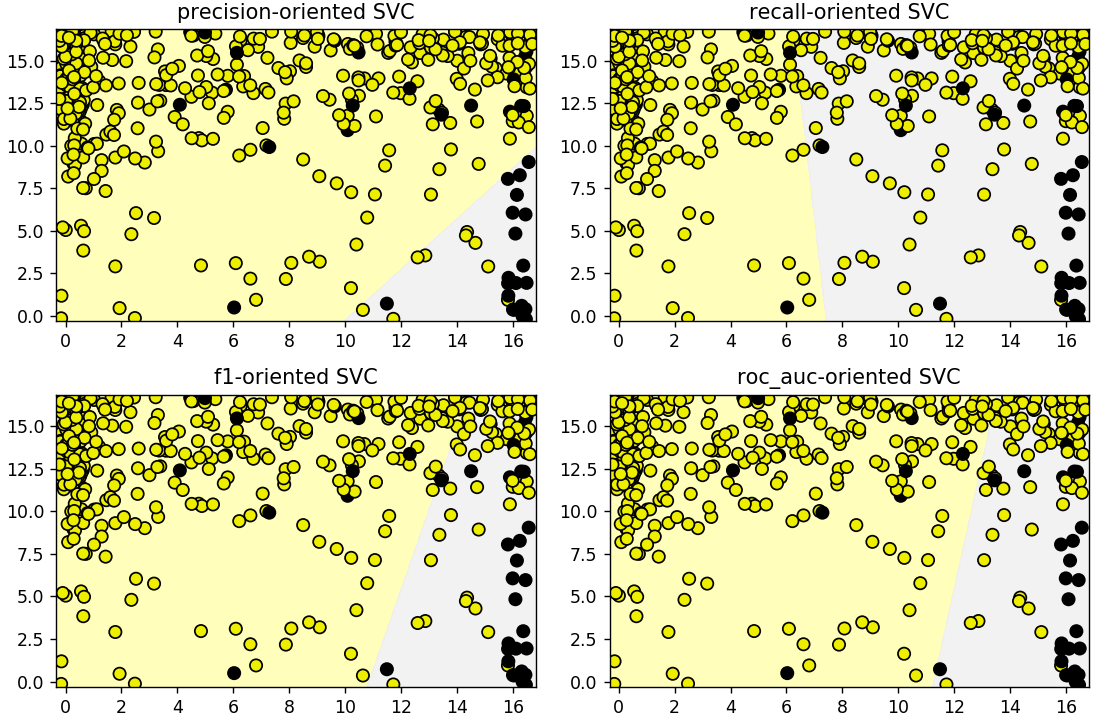
\includegraphics[width=\linewidth]{img/Optimizing-Classifier.png} 
\end{center}


In these classification visualization examples, the positive examples, the digit one are shown as black points and the region of positive class prediction is shown in the light-colored or yellow region to the right of this decision boundary. The negative examples, all other digits, are shown as white points. And the region of negative class prediction here in these figures is to the left of the decision boundary. The data points have been plotted using two out of the 64 future values in the digits' dataset and have been jittered a little. That is, I've added a little bit of random noise so we can see more easily the density of examples in the feature space. 

Here's the scikit-learn code that produced this figure. We apply grid search here to explore different values of the optional class weight parameter that controls how much weight is given to each of the two classes during training. As it turns out, optimizing for different evaluation metrics results in different optimal values of the class weight parameter. As the class weight parameter increases, more emphasis will be given to correctly classifying the positive class instances. 

%\begin{center}
%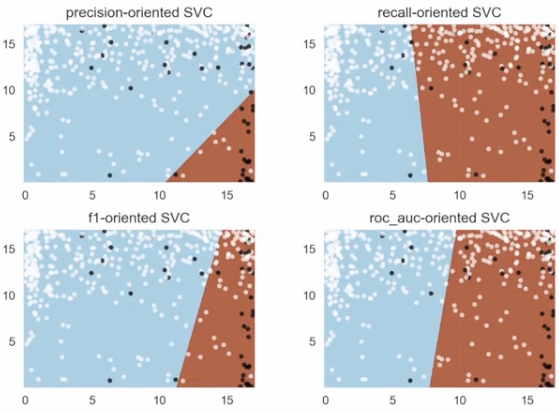
\includegraphics[width=\linewidth]{img/Optimizing-Classifier2.png} 
%\end{center}

The precision-oriented classifier we see here with class weight of two, tries hard to reduce false negatives while increasing true positives. So it focuses on the cluster of positive class points in the lower right corner where there are relatively few negative class points. Here, precision is over 50 percent. 

In contrast, the recall-oriented classifier with class weight of 50, tries hard to reduce the number of false negatives while increasing true positives. That is, it tries to find most of the positive class points as part of its positive class predictions. We can also see that the decision boundary for the F1-oriented classifier has an optimal class weight of two, which is between the optimal class weight values for the precision and recall-oriented classifiers. Visually we can see that the F1-oriented classifier also has a kind of intermediate positioning between the precision and recall-oriented, decision boundaries. This makes sense given that F1 is the harmonic mean of precision and recall. 

The AUC-oriented classifier with optimal class weight to 5 has a similar decision boundary to the F1-oriented classifier, but shifted slightly in favor of higher recall. We can see the precision recall trade-off very clearly for this classification scenario in the precision recall curve for the default support vector classifier with linear kernel optimized for accuracy on the same dataset, and using the balanced option for the class weight parameter. Let's take a look at the code that generated this plot. Take a moment to imagine how the extreme lower right part of the curve on this precision recall curve represents a decision boundary that's highly precision-oriented in the lower right of the classification plot, where there's a cluster of positive examples. 

As the decision threshold is shifted to become less and less conservative, tracing the curve up into the left, the classifier becomes more and more like the recall-oriented support vector classifier example. Again, the red circle represents the precision recall trade-off achieved at the zero score mark, which is the actual decision boundary chosen for the trained classifier. 

For simplicity, we've often used a single train-test split in showing examples of evaluation scoring. However, using only cross-validation or a test set for model selection or parameter tuning may still lead to more subtle forms of overfitting and less optimistic evaluation estimates for future, unseen data. An intuitive explanation for this might be the following: "remember that the whole point of evaluating on a test set is to estimate how well a learning algorithm might perform on future, unseen data. 

The more information we see about our dataset as part of repeated cross-validation passes in choosing our model, the more influence any potential held-up test data has played into selecting the final model. Not merely evaluating it. This is sometimes called data leakage and we'll describe more about that phenomenon in another module. So, we haven't done an evaluation with a truly held-out test set unless we commit to holding back a test split that isn't seen by any process until the very end of the evaluation. 

So that's what's actually done in practice. There are three data splits: training for model building, validation for model selection and a test set for the final evaluation. The training and test sets are typically split out first, and then cross-validation is run using the training data to do model and parameter selection. Again, the test set is not seen until the very end of the evaluation process. Machine learning researchers take this protocol very seriously. The train-validate-test design is a very important universally applied framework for effective evaluation of machine learning models. 

\section{Conclusion}

That brings us to the end of this section of the course on evaluation for machine learning. You should now understand why accuracy only gives a partial picture of a classifier's performance and be more familiar with the motivation and definition of important alternative evaluation methods and metrics of machine learning like confusion matrices, precision, recall, F1 score and area under the RAC curve. 
You've also seen how to apply and choose these different evaluation metric alternatives in order to optimize model selection or parameter tuning for a classifier, to maximize a given evaluation metric. 

Finally, I'd like to leave you with a couple of points. First, simple accuracy may not often be the right goal for your particular machine learning application. As we saw for example with tumor detection or credit card fraud, false positives and false negatives might have very different real-world effects for users or for organization outcomes. So it's important to select an evaluation metric that reflects those user application or business needs. 

Second, there are a number of other dimensions along which it may be important to evaluate your machine learning algorithms, that we don't cover here but that are important for you to be aware of. I'll mention two specifically here. Learning curves are used to assess how a machine learning algorithm's evaluation metric changes or improves as the algorithm gets more training data. Learning curves may be useful as part of a cost-benefit analysis. Gathering training data in the form of labeled examples is often time-consuming and expensive. So being able to estimate the likely performance improvement of your classifier, if you say invest in doubling the amount of training data, can be a useful analysis. Second, sensitivity analysis amounts to looking at how an evaluation metric changes as small adjustments are made to important model parameters. This helps assess how robust the model is to choice of parameters. 

This may be important to perform especially if there are other costs such as runtime efficiency that are critical variables when deploying an operational system, that are correlated with different values of parameter. For example, decision tree depth or future value threshold. In this way, a more complete picture of the trade-offs achievable across different performance dimensions can help you make the best practical deployment decisions for your machine learning model. 

\end{multicols}

\end{multicols}
\end{document}